\section{Circuito Pasabajos}
En esta secci\'on se realizar\'a el an\'alisis de un circuito de segundo orden configurado de forma tal,
que la salida tiene un comportamiento denominado como filtro pasabajos, debido a que como se observar\'a en el an\'alisis,
\'unicamente permite pasar las bajas frecuencias.

En primer lugar se llevar\'a a cabo un an\'alisis te\'orico para estudiar el comportamiento del circuito, luego se realizar\'an mediciones
y simulaciones de ser necesario, contrastando los resultados pr\'acticos con las estimaciones te\'oricas en base a los modelos empleados. Adem\'as,
los componentes que se pueden observar en la figura \ref{fig:circuito_pasabajos} est\'an dados como $L = 500 \mu H$, $C = 22nF$ y se desea que el sistema
est\'e caracterizado con un coeficiente de amortiguamiento $\xi = 0,4$.

\begin{figure}[H]
    \centering
    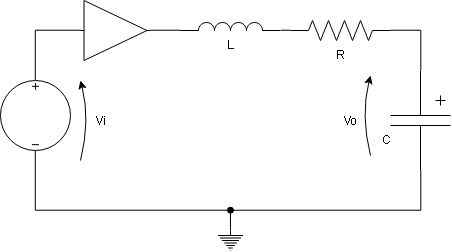
\includegraphics[scale=0.5]{Recursos/circuito_pasabajos.png}
    \caption{Circuito pasabajos}
    \label{fig:circuito_pasabajos}
\end{figure}

\subsection{An\'alisis te\'orico}

\subsubsection{Funci\'on transferencia}
El circuito a estudiar en este an\'alisis, est\'a compuesto por un buffer implementado utiizando un amplificador operacional y
tres componentes pasivos, estos son, una resistencia, un capacitor y un inductor. Para estudiar el circuito es necesario comenzar caracterizandolo
a trav\'es de la funci\'on tranferencia, para lo cual se asume que el mismo es un sistema lineal, de tiempo invariante, causal y bibo-estable. Adem\'as,
se consideran el capacitor y el inductor ideales, sin tener en cuenta los efectos adicionales que deban incorporarse por sus caracter\'isticas constructivas en
la realidad. Con estas consideraciones en mente, se aplica un divisor de tensi\'on para obtener la $H(s) = \frac{V_o(s)}{V_i(s)}$.

\begin{align*}
    & V_o = V_i \cdot \frac{\frac{1}{s \cdot C}}{s \cdot L + R + \frac{1}{s \cdot C}} \\
    & \Rightarrow
    V_o = \frac{V_i}{1 + s \cdot (C \cdot R) + s^{2} \cdot (L \cdot C)}
\end{align*}

\begin{align}
    H(s) &= \frac{V_o}{V_i} = \frac{1}{1 + \frac{2 \cdot \xi \cdot s}{\omega_o} + \left( \frac{s}{\omega_o} \right)^{2}}
    \label{eq:Trans_PB}
    \\
    \omega_o &= \frac{1}{ \sqrt{(L \cdot C)} } \\
    \xi &= \frac{R}{2} \cdot \sqrt{\frac{C}{L}} 
\end{align}


Vale mencionar, que el t\'ermino lineal del polinomio cuadr\'atico, adem\'as de poder ser expresado como $\frac{2 \cdot \xi}{\omega_o}$ puede
ser expresado en funci\'on del factor de calidad Q del sistema, que describe la relaci\'on (temporalmente hablando) entre el tiempo de establecimiento
y la frecuencia natural del sistema, o bien desde un punto de vista de frecuencias define el cociente entre la frecuencia de resonancia y el ancho de banda.
Entonces, tambi\'en se puede caracterizar dicho par\'ametro:

\begin{equation}
    Q = \frac{\omega_o}{\Delta \omega} = \frac{1}{2 \cdot \xi}
\end{equation}

Dado que est\'a consignado el valor del coeficiente de amortiguamiento del sistema, luego se puede obtener en t\'erminos ideales el valor de la resistencia
para alcanzar tal estado, con lo cual despejando se obtiene que la resistencia debiera de tener un valor de $R = 120.6 \Omega$. Esto en la pr\'actica no ser\'a necesariamente
as\'i puesto que los modelos pr\'acticos para el capacitor y el inductor, desviar\'an el verdadero valor que deber\'a tomar la resistencia
para que se pueda observar ese comportamiento. Es por esto \'ultimo que si bien en el desarrollo te\'orico se considera una resistencia de tal valor, en la pr\'actica se buscar\'a
llevar al sistema hasta tal estado, utilizando para ello una resistencia variable que lo permita. Entonces el sistema tiene una frecuencia angular de resonancia natural $\omega_o = 301511,34 \frac{1}{s} = 2 \pi \cdot 47,987kHz$.

Analizando el circuito en el dominio de las frecuencias, por tener un valor de $\xi = 0,4 < 1$ se dice que el sistema se encuentra subamortiguado, con lo cual observando la funci\'on transferencia se 
llega a que posee dos polos complejos y conjugados, y la respuesta en frecuencia seg\'un lo asumido anteriormente deber\'ia tener un sobrepico en una frecuencia previa a la frecuencia de corte o resonancia natural y decaer
40 decibeles por d\'ecada a partir de dicha frecuencia. Esto se puede observar en los diagramas de la Fig. \ref{fig:bode_teorico}.

\begin{figure}[H]
    \centering
    \begin{tabular}{c c}
        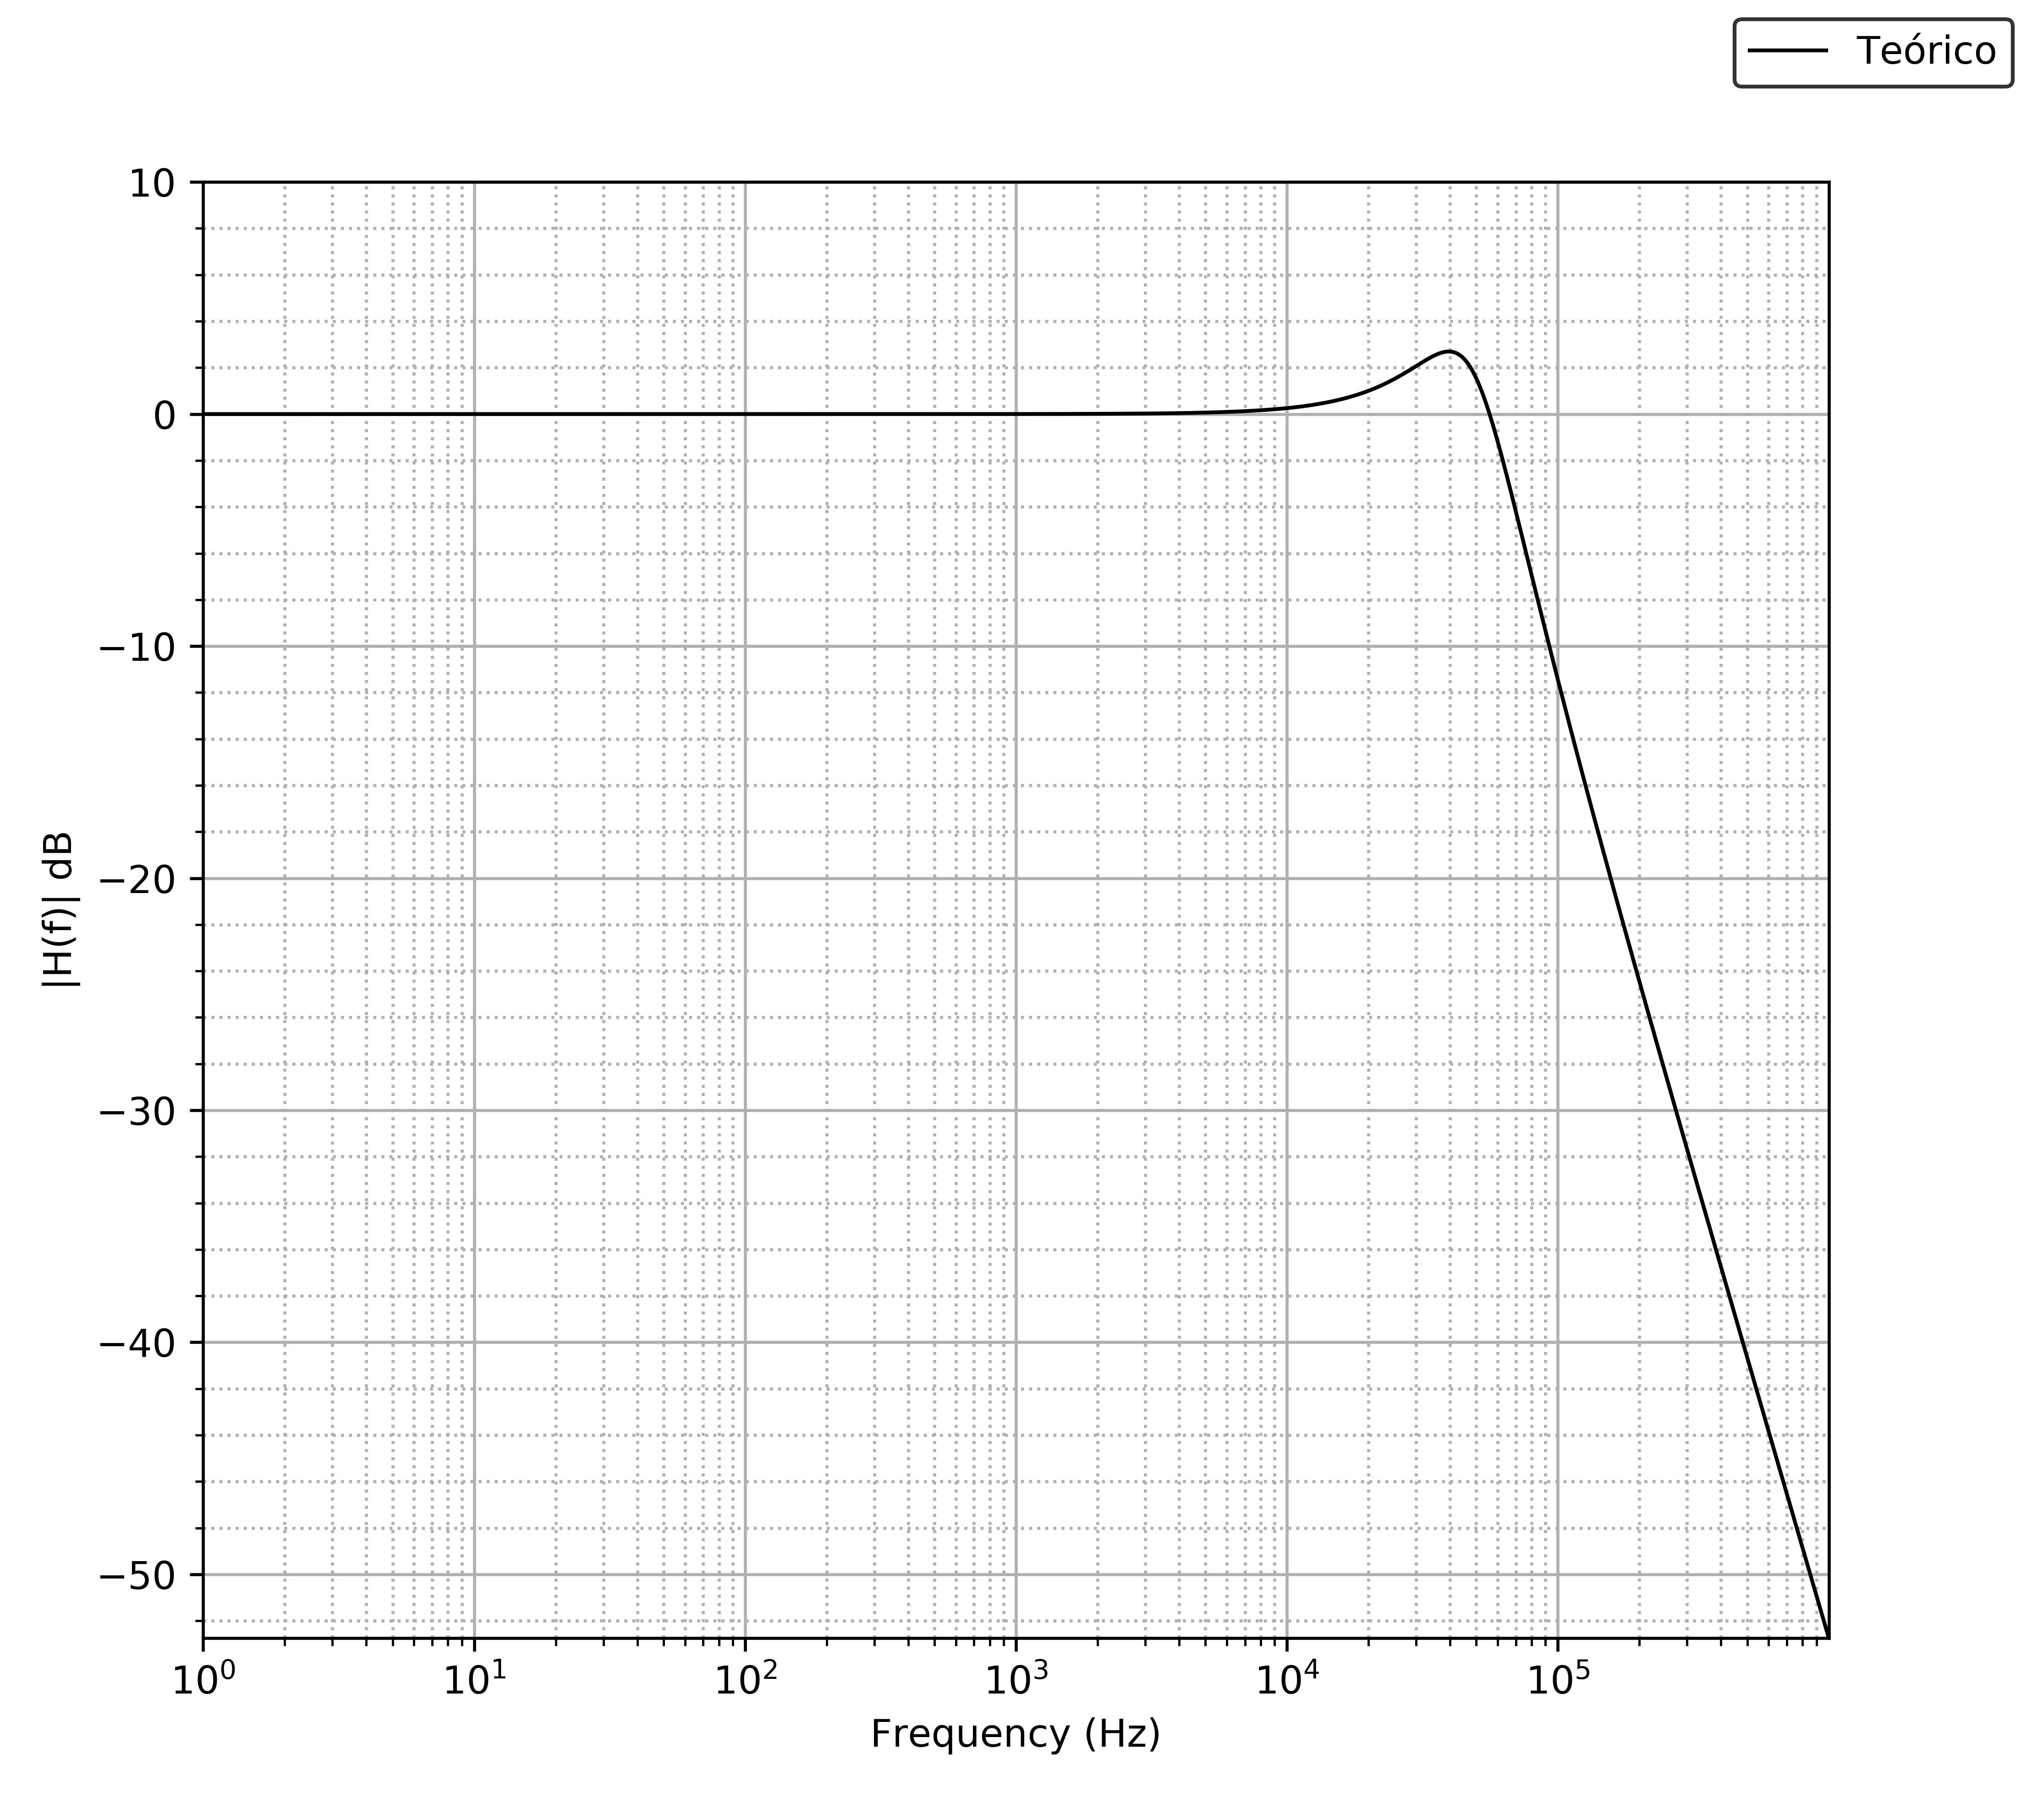
\includegraphics[scale=0.4]{Recursos/bode_teorico_pasabajos_modulo.png}
        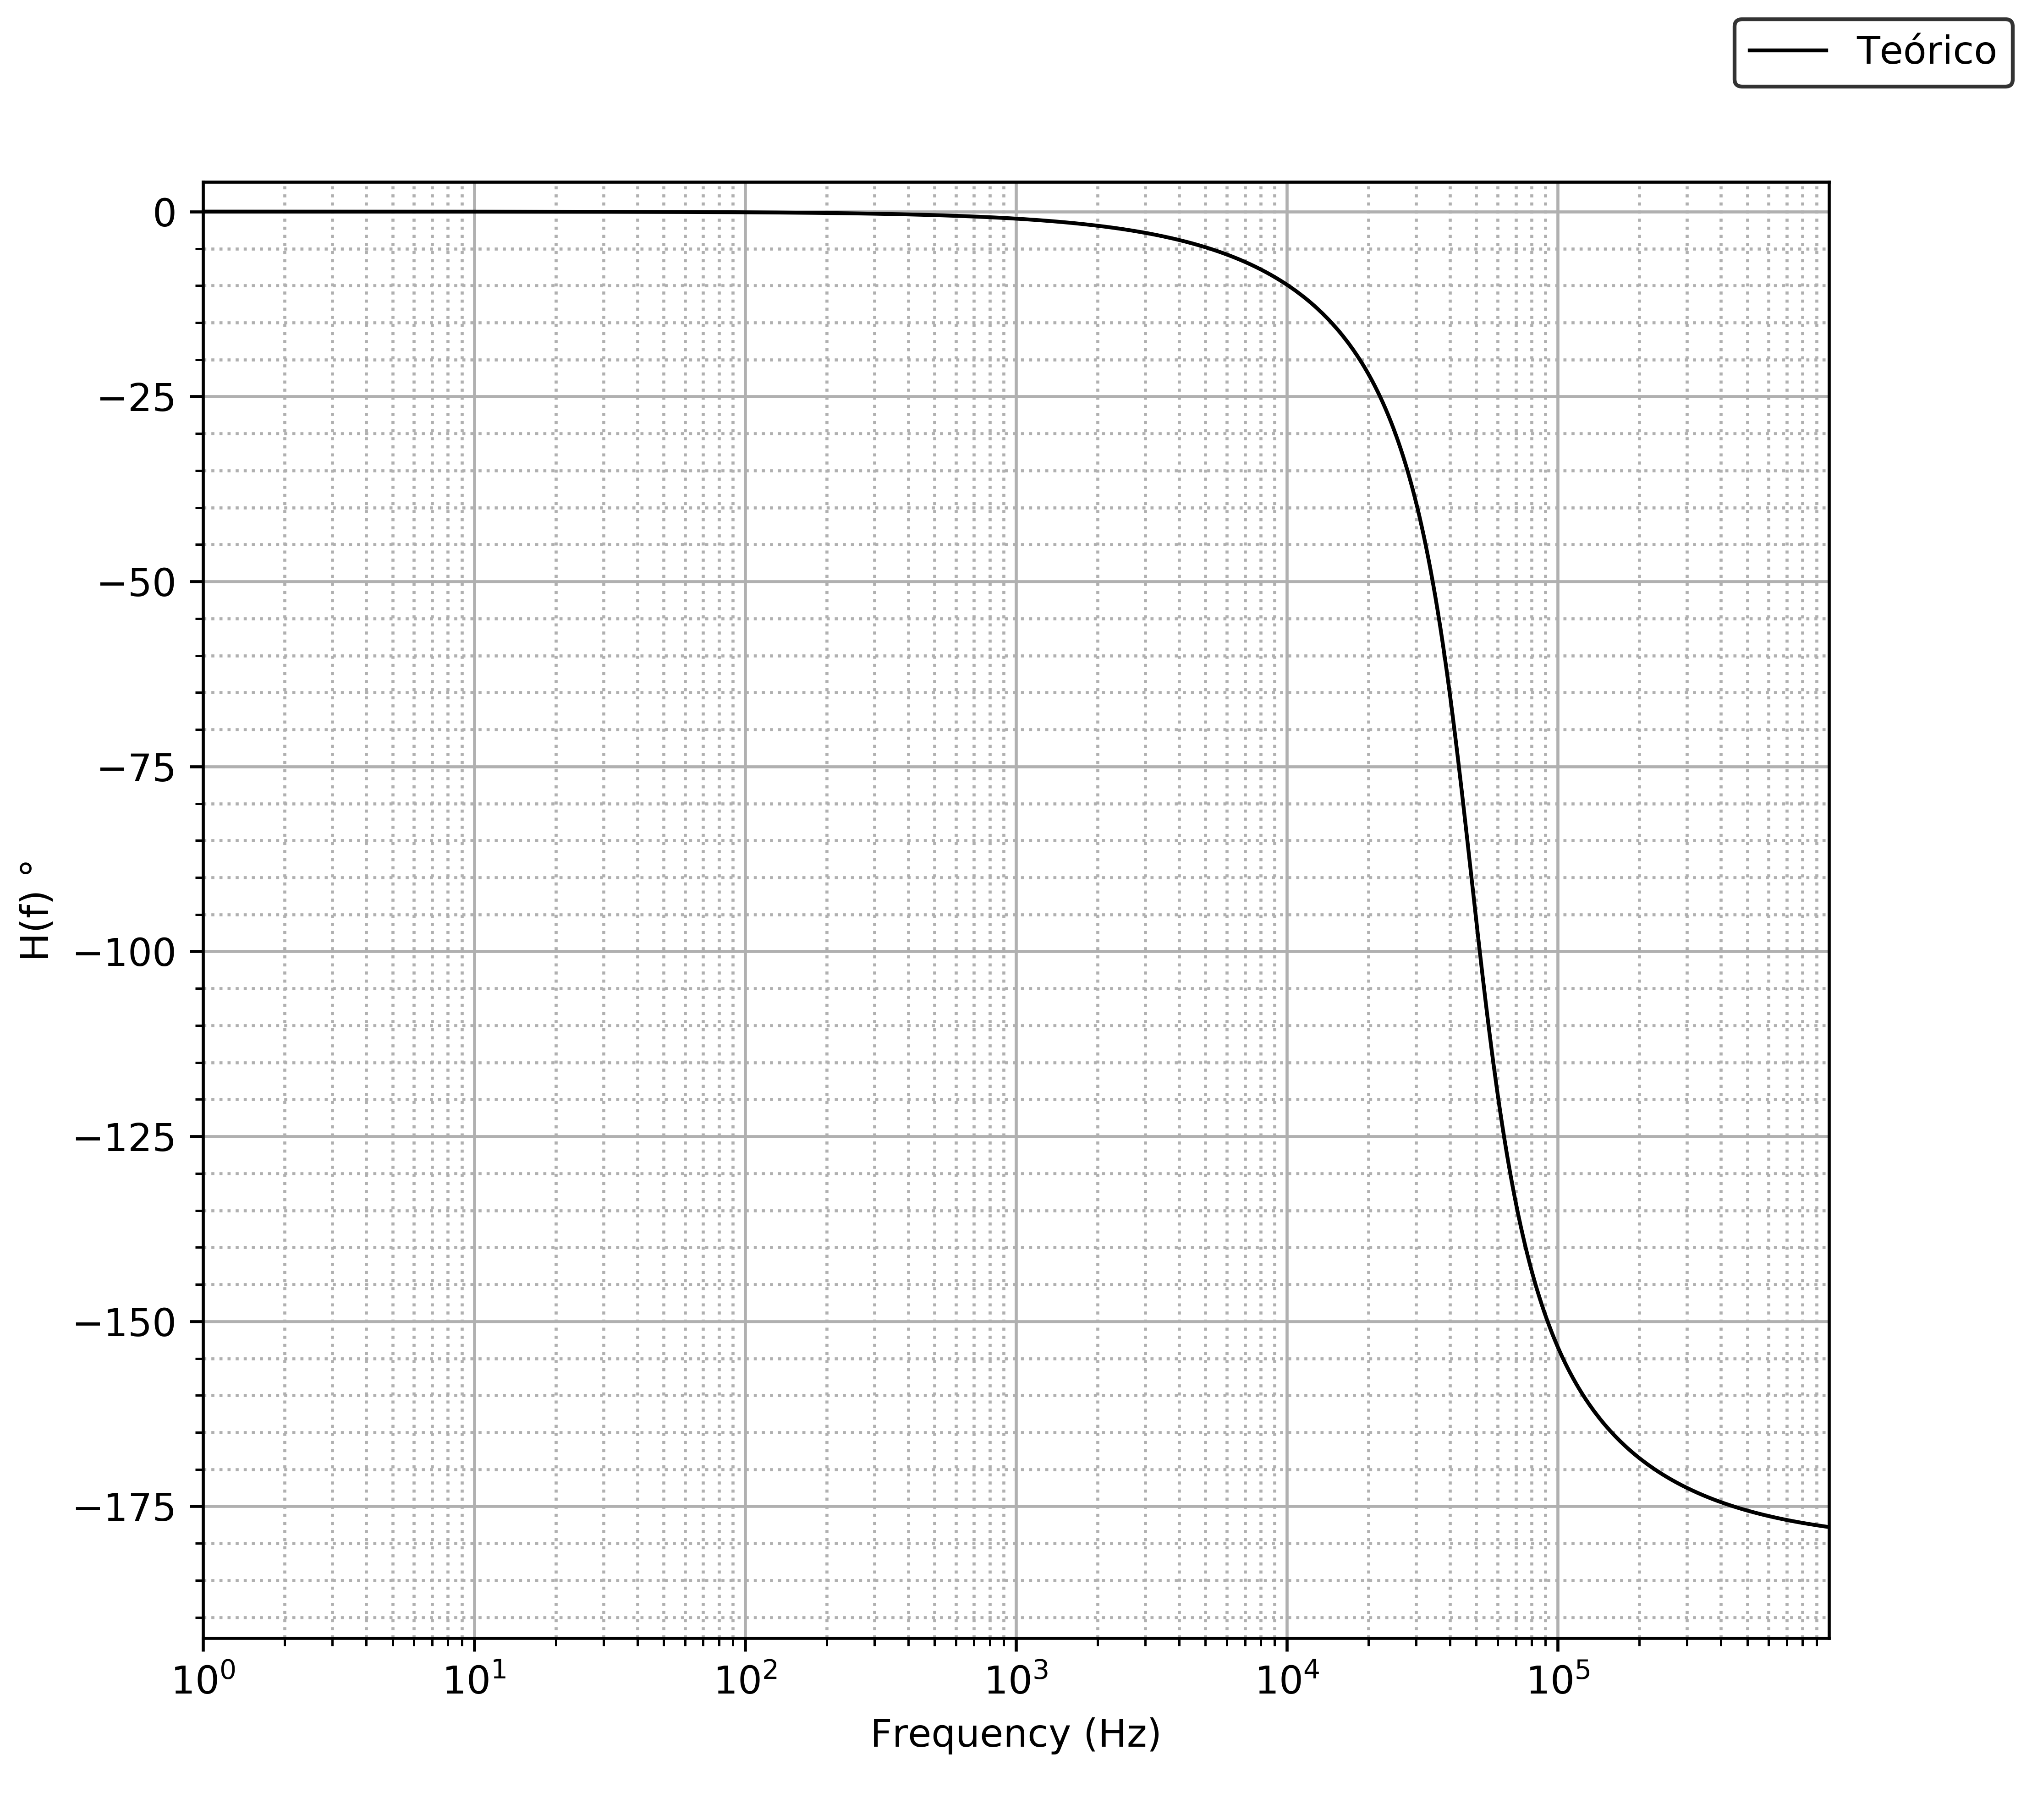
\includegraphics[scale=0.4]{Recursos/bode_teorico_pasabajos_fase.png}
    \end{tabular}
    \caption{Diagramas de bode $H(s=2\pi \cdot f)$ te\'orico}
    \label{fig:bode_teorico}
\end{figure}

Analizando el circuito en el dominio del tiempo, se busca la respuesta del sistema a un escal\'on de amplitud arbitraria que luego en la pr\'actica se ver\'a definida en base a 
algunas limitaciones que puedan darse f\'isicamente. Para esto se considera una se\~nal entrante al sistema de la forma de $V_i(s) = \frac{A}{s}$ y si se reacomodan con algunos pasos 
algebraicos algunos t\'erminos, luego se puede obtener tal respuesta antitransformando por laplace al dominio temporal.

\begin{align*}
    & V_o(s) = V_i(s) \cdot H(s) = \frac{A}{s} \cdot \frac{\omega_o}{\sqrt{1 - \xi^{2}}} \cdot \frac{\omega_o \cdot \sqrt{1 - \xi^{2}}}{(s + \xi \cdot \omega_o)^{2} + (\omega_o \cdot \sqrt{1 - \xi^{2}})^{2}} \\
    & \Rightarrow
    v_o(t) = A \cdot \left[ 1 - \frac{e^{-\alpha \cdot t}}{\sqrt{1 - \xi^{2}}} \cdot \sin{(\omega_d \cdot t + \theta)}\right] \\
    & \omega_d = \omega_o \cdot \sqrt{1 - \xi^{2}} \\
    & \alpha = \xi \cdot \omega_o \\
    & \theta = \arctan{(\frac{\omega_d}{\alpha})}
\end{align*}

\subsubsection{Valores caracter\'isticos de transitorio}
En el caso del dominio temporal, la $\omega_o$ es llamada frecuencia angular natural, y cuando el sistema se encuentre en un estado subamortiguado como sucede aqu\'i, en la respuesta natural o en la transitoria se 
observar\'a una oscilaci\'on amortiguada, es decir, cuya amplitud va disminuyendo a medida que pasa al tiempo. Para esta oscilaci\'on se define la frecuencia amortiguada (la llamada frecuencia del transitorio) como $f_d = \frac{\omega_d}{2 \pi} = 43,98kHz$.
Por otro lado, tambi\'en se puede estimar a partir de la anterior expresi\'on el valor del tiempo de establecimiento para el cual se considera que el transitorio est\'a terminando, para esto se toma como criterio el punto en el cual
la oscilaci\'on amortiguada o bien su envolvente, est\'a dentro de un margen del $5 \%$ respecto de la amplitud del escal\'on.

\begin{equation}
    \frac{e^{- \alpha \cdot t_s}}{\sqrt{1 - \xi^{2}}} = 0.05 
    \Rightarrow
    t_s = \frac{\ln{(0.05 \cdot \sqrt{1 - \xi^{2}})}}{- \alpha} = 25.56 \mu s
\end{equation}

Finalmente, si se toma la se\~nal $v_o(t)$ y se la deriva buscando un punto cr\'itico que sea m\'aximo, luego se puede obtener la ubicaci\'on temporal y la magnitud del sobrepico,
es decir, dentro de las oscilaciones del transitorio, cu\'al es la de mayor valor pico.

\begin{equation}
    \frac{\delta v_o (t_p)}{\delta t} = 0 
    \Leftrightarrow
    - \alpha \cdot \sin{(\omega_d \cdot t_p + \theta)} + \omega_d \cdot \cos{(\omega_d \cdot t_p + \theta)} = 0
    \Leftrightarrow
    t_p = \frac{\pi}{\omega_d}
\end{equation}

\begin{equation}
    v_o(t_p) = A  \cdot (1 + e^{\frac{- \xi \cdot \pi}{\sqrt{1 - \xi^{2}}}})
    \Rightarrow 
    M_p = \frac{vo_{max} - A}{A} = e^{\frac{- \xi \cdot \pi}{\sqrt{1 - \xi^{2}}}} = 0,253
\end{equation}

Teniendo en cuenta que se utilizar\'a una se\~nal de escal\'on con una amplitud de $A = 1V_{pp}$, luego se observa el sobrepico en la respuesta transitoria
del sistema en el valor $t_p = 11.368 \mu s$ con una magnitud de $v_o(t_p) = 1.25 V$.

\subsubsection{An\'alisis de casos}
A continuaci\'on se aplican los desarrollos matem\'aticos obtenidos del estudio del sistema propuesto a diferentes casos, y para cada uno de ellos
se obtienen las variables o estados caracter\'isticos, present\'andolos en la Tabla \ref{tab:tabla_casos_pasabajo}.

\begin{table}[H]
    \centering
    \begin{tabular}{c c c c c c c c c}
        $R$ & $\xi$ & $f_d$ & $t_s$ & $t_p$ & $M_p$ & $Sistema$ \\
        \hline \\
        $120.6 \Omega$ & $0.4$ & $43.98kHz$ & $25.56 \mu s$ & $11.368 \mu s$ & $0.253$ & $Subamortiguado$ \\
        $155.86 \Omega$ & $0.51693$ & $41.078kHz$ & $20.218 \mu s$ & $12.171 \mu s$ & $0.15$ & $Subamortiguado$ \\
        $0 \Omega$ & $0$ & $47.98kHz$ & $-$ & $-$ & $-$ & $Oscila$ \\
        $301.511 \Omega$ & $1$ & $0Hz$ & $-$ & $-$ & $-$ & $Criticamente        $ \\
        \hline
    \end{tabular}
    \caption{Casos del circuito pasabajos}
    \label{tab:tabla_casos_pasabajo}
\end{table}

Para el primero de los casos, se busca que el sobrepico tenga un valor de $M_p = 0.15$ para ello se aplica la ecuaci\'on antes despejada, de la cual
se obtiene la siguiente relaci\'on.

\begin{align}
    & M_p = e^{\frac{- \xi \cdot \pi}{\sqrt{1 - \xi^{2}}}}
    \Rightarrow
    \xi = \sqrt{ \frac{K^{2}}{1 + K^{2}} } , 
    K = \frac{ \ln{(M_p)}}{\pi} \\
    & \Rightarrow \xi = 0.51693 \Rightarrow R = 155.86 \Omega
\end{align}

Por otro lado, si se impone que en un caso ideal donde no haya presencia de resistencia del generador, ni del bobinado, el capacitor o los cables,
luego considerando que $ R = 0 \Omega$ entonces se obtiene que el sistema se encuentra en una oscilaci\'on puesto que $\xi = 0$, con lo cual la componente 
de amortiguamiento de la respuesta transitoria no est\'a, y la oscilaci\'on perdura idealmente para siempre. En este caso, la frecuencia de oscilaci\'on observada deber\'ia
ser la natural, es decir, $f_o = \frac{\omega_o}{2 \pi} = 47,987kHz$.

Finalmente, si se busca que el sistema se encuentre cr\'iticamente amortiguado estableciendo que $\xi = 1$, entonces la resistencia debiera de valer idealmente $R = 301,511 \Omega$. Los dem\'as valores
que caracterizan al sistema para cada caso, son calculados directamente empleando las expresiones ya mostradas con anterioridad. No obstante esto, para el caso donde el sistema deber\'ia oscilar no tiene
sentido calcular algunos de los par\'ametros, por lo tanto se los dej\'o vac\'ios.

\subsection{Resultados}
En la secci\'on de resultados, se toman resultados de las mediciones del circuito tanto desde un aspecto temporal como es con la respuesta transitoria como lo es en frecuencia,
con el caso de la respuesta en frecuencia. Para ello, se consideran diferentes casos del circuito que fueron mencionados inicialmente en el an\'alisis te\'orico del circuito, y 
consisten en:

\begin{itemize}
    \item Circuito con $\xi = 0.4$
    \item Circuito con $M_p = 0.15$
    \item Circuito con $R = 0 \Omega $
    \item Circuito con un estado cr\'iticamente amortiguado
    \item Circuito con $M_p = 0.15$ sin buffer
    \item Circuito con $R = 0 \Omega$ sin buffer
\end{itemize}

\subsubsection{Mediciones del transitorio}
En correspondiente con lo ya introducido anteriormente, a continuaci\'on se presentan los resultados de las mediciones para cada caso, vale mencionar que para cumplir con aquellos donde lo que se pauta
es alg\'un par\'ametro caracter\'istico del circuito, se emple\'o una resistencia variable con el fin de poder ajustar el valor de tal caracter\'istica a lo consignado, para de esa forma realizar mediciones que 
fueran bajo la condici\'on requerida. Es por esto \'ultimo, que para los casos que requirieron de tal proceso de calibraci\'on del circuito, se midi\'o el valor de resistencia del preset utilizado para 
poder ponerlo bajo an\'alisis posteriormente.

Vale aclarar, que en la tabla se llaman $f_t$ a la frecuencia amortiguada del transitorio, $t_s$ al tiempo de establecimiento, $t_p$ al tiempo al pico desde que inicia el transitorio, 
$M_p$ al valor del sobrepico relativo al estado de r\'egimen permanente y, finalmente, $R$ la resistencia del circuito.

\begin{table}[H]
    \centering
    \begin{tabular}{c c c c c c}
        $Caso$ & $f_T$ & $t_s$ & $t_p$ & $M_p$ & $R$ \\
        \hline \\
        $\xi = 0.4$ & $46.083kHz$ & $25.6\mu s$ & $11.1\mu s$ & $0.25$ & $113.2 \Omega$ \\
        $M_p = 0.15$ & $41.15kHz$ & $17.6 \mu s$ & $12.1\mu s$ & $0.15$ & $148.3 \Omega$ \\
        $R = 0\Omega$ & $49.505kHz$ & $90.4 \mu s$ & $10.4 \mu s$ & $0.7125$ & $0 \Omega$ \\
        $\xi = 1$ & $-$ & $29.2 \mu s$ & $-$ & $-$ & $291 \Omega$ \\
        $M_p = 0.15$ sin buffer & $41.528kHz$ & $17.4 \mu s$ & $11.7 \mu s$ & $0.15$ & $97.5 \Omega$ \\
        $R = 0\Omega$ sin buffer & $49.02kHz$ & $40.7 \mu s$ & $9.9 \mu s$ & $0.48$ & $0 \Omega$ \\
        \hline
    \end{tabular}
\end{table}

Para tomar tales mediciones, se muestran a continuaci\'on las capturas de pantalla del osciloscopio para el caso
en el cual la resistencia ten\'ia un valor $R = 0 \Omega$.

\begin{figure}[H]
    \centering
    \begin{tabular}{c c}
        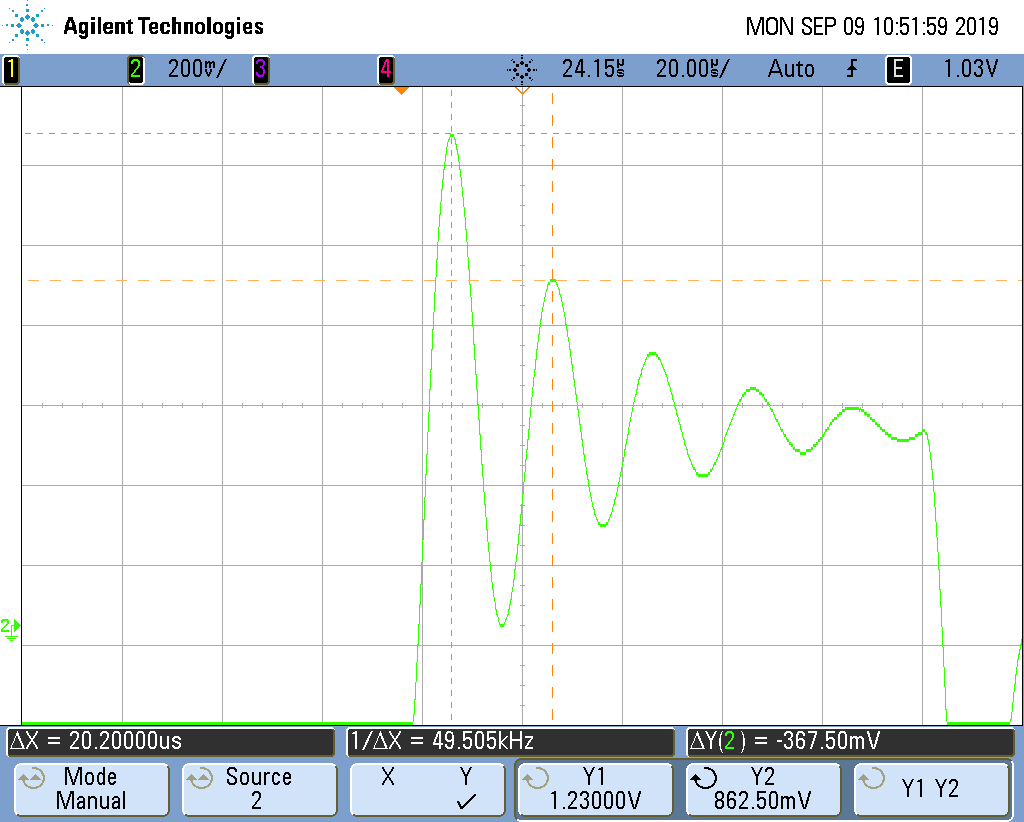
\includegraphics[scale=0.2]{../Mediciones/Osciloscopio/Pasabajos_respuesta_caso_0/scope_9.png} &
        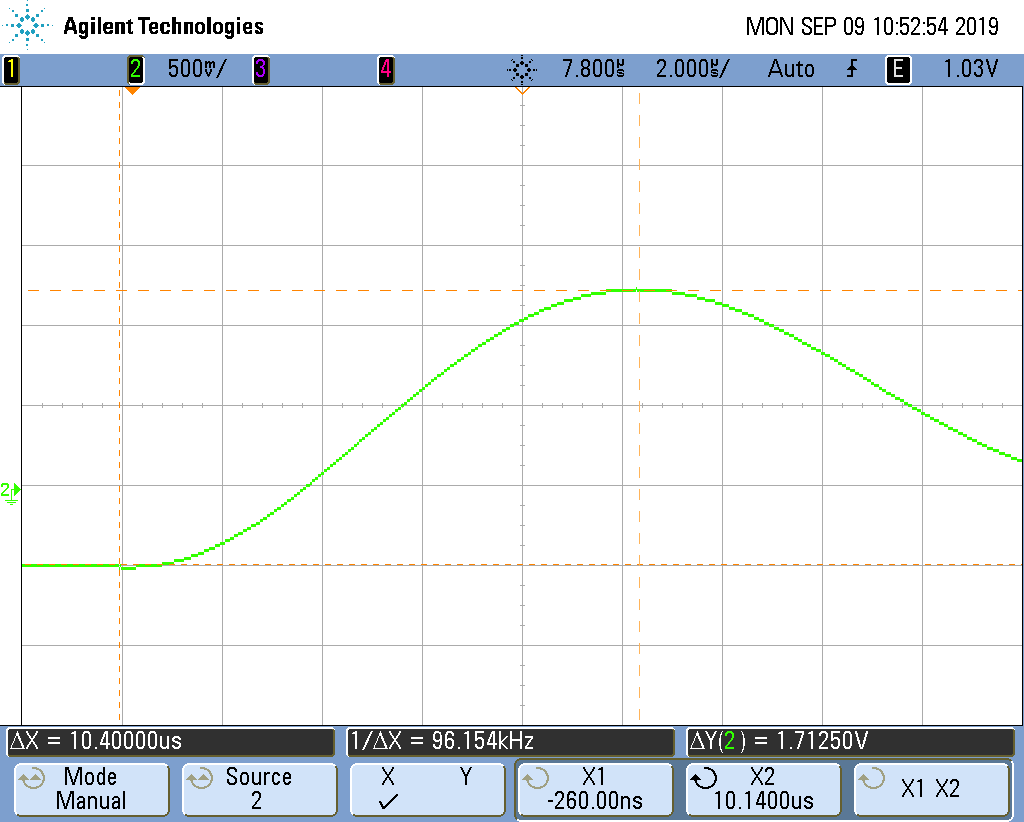
\includegraphics[scale=0.2]{../Mediciones/Osciloscopio/Pasabajos_respuesta_caso_0/scope_10.png} \\
    \end{tabular}
    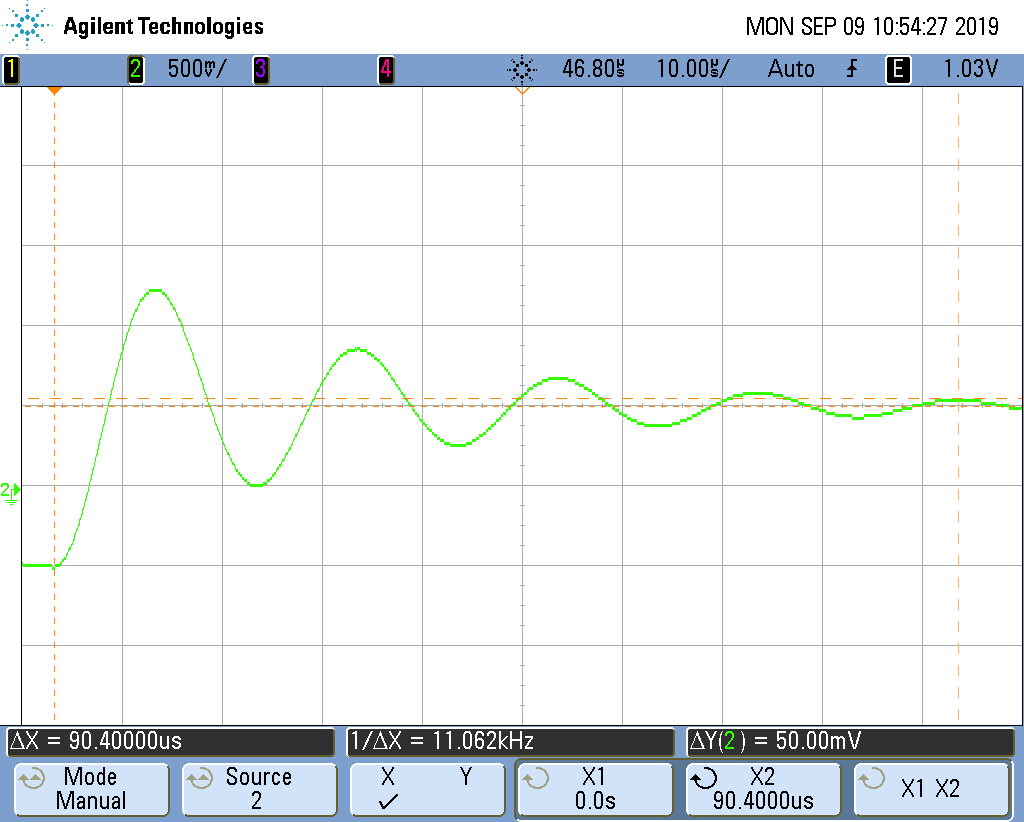
\includegraphics[scale=0.2]{../Mediciones/Osciloscopio/Pasabajos_respuesta_caso_0/scope_11.png} 
    \caption{Mediciones de pico, establecimiento y frecuencia}
    \label{fig:transitorio_pasabajos}
\end{figure}

En el siguiente an\'alisis se hace alusi\'on a los resultados de la Tabla \ref{fig:transitorio_pasabajos}, de donde se pueden destacar algunos aspectos interesantes. En primer lugar,
se puede observar que para el caso con y sin buffer, donde se ajusta el valor de la resistencia variable del preset para cumplir con la condici\'on de 
sobrepico, los resultados medidos sobre el preset var\'ian entre uno y otro caso y tiene que ver con la adaptaci\'on de impedancia que realiza el buffer,
puesto que cuando se lo quita aparece la resistencia del generador en serie $R_{gen} = 50 \Omega$, lo cual es una diferencia coherente entre los valores medidos.
Por otro lado para el caso donde la $R = 0 \Omega$, a diferencia de lo que se esperar\'ia desde un punto de vista ideal donde el circuito debiera de oscilar,
se presenta un subamortiguamiento muy fuerte que eventualmente se desvanece, esto se debe a que por m\'as que la resistencia que coloquemos sea nula, est\'an presentes
las resistencias del capacitor, el bobinado, el cable, la de salida del amplificador operacional que no es ideal, entre otras cosas.
Finalmente, la presencia de estas resistencias "par\'asitas" que se mencionaron recien sumado a las variaciones en la tolerancia de una resistencia, fueron las razones iniciales por las cuales
se utiliz\'o un preset para poder establecer la condici\'on del sistema. No obstante, existe una diferencia entre el valor te\'orico y el valor real de tal resistencia, donde la teor\'ia indicaba
que la resistencia deber\'ia ser de $R \approx 120 \Omega$ y termin\'o siendo de $R = 113.2 \Omega$ en la pr\'actica, esto se atribuye a los efectos ya mencionados de resistencias que mueven el valor total
en serie.

\subsubsection{Medici\'on de respuesta en frecuencia}

\begin{figure}[H]
    \centering
    \begin{tabular}{c c}
        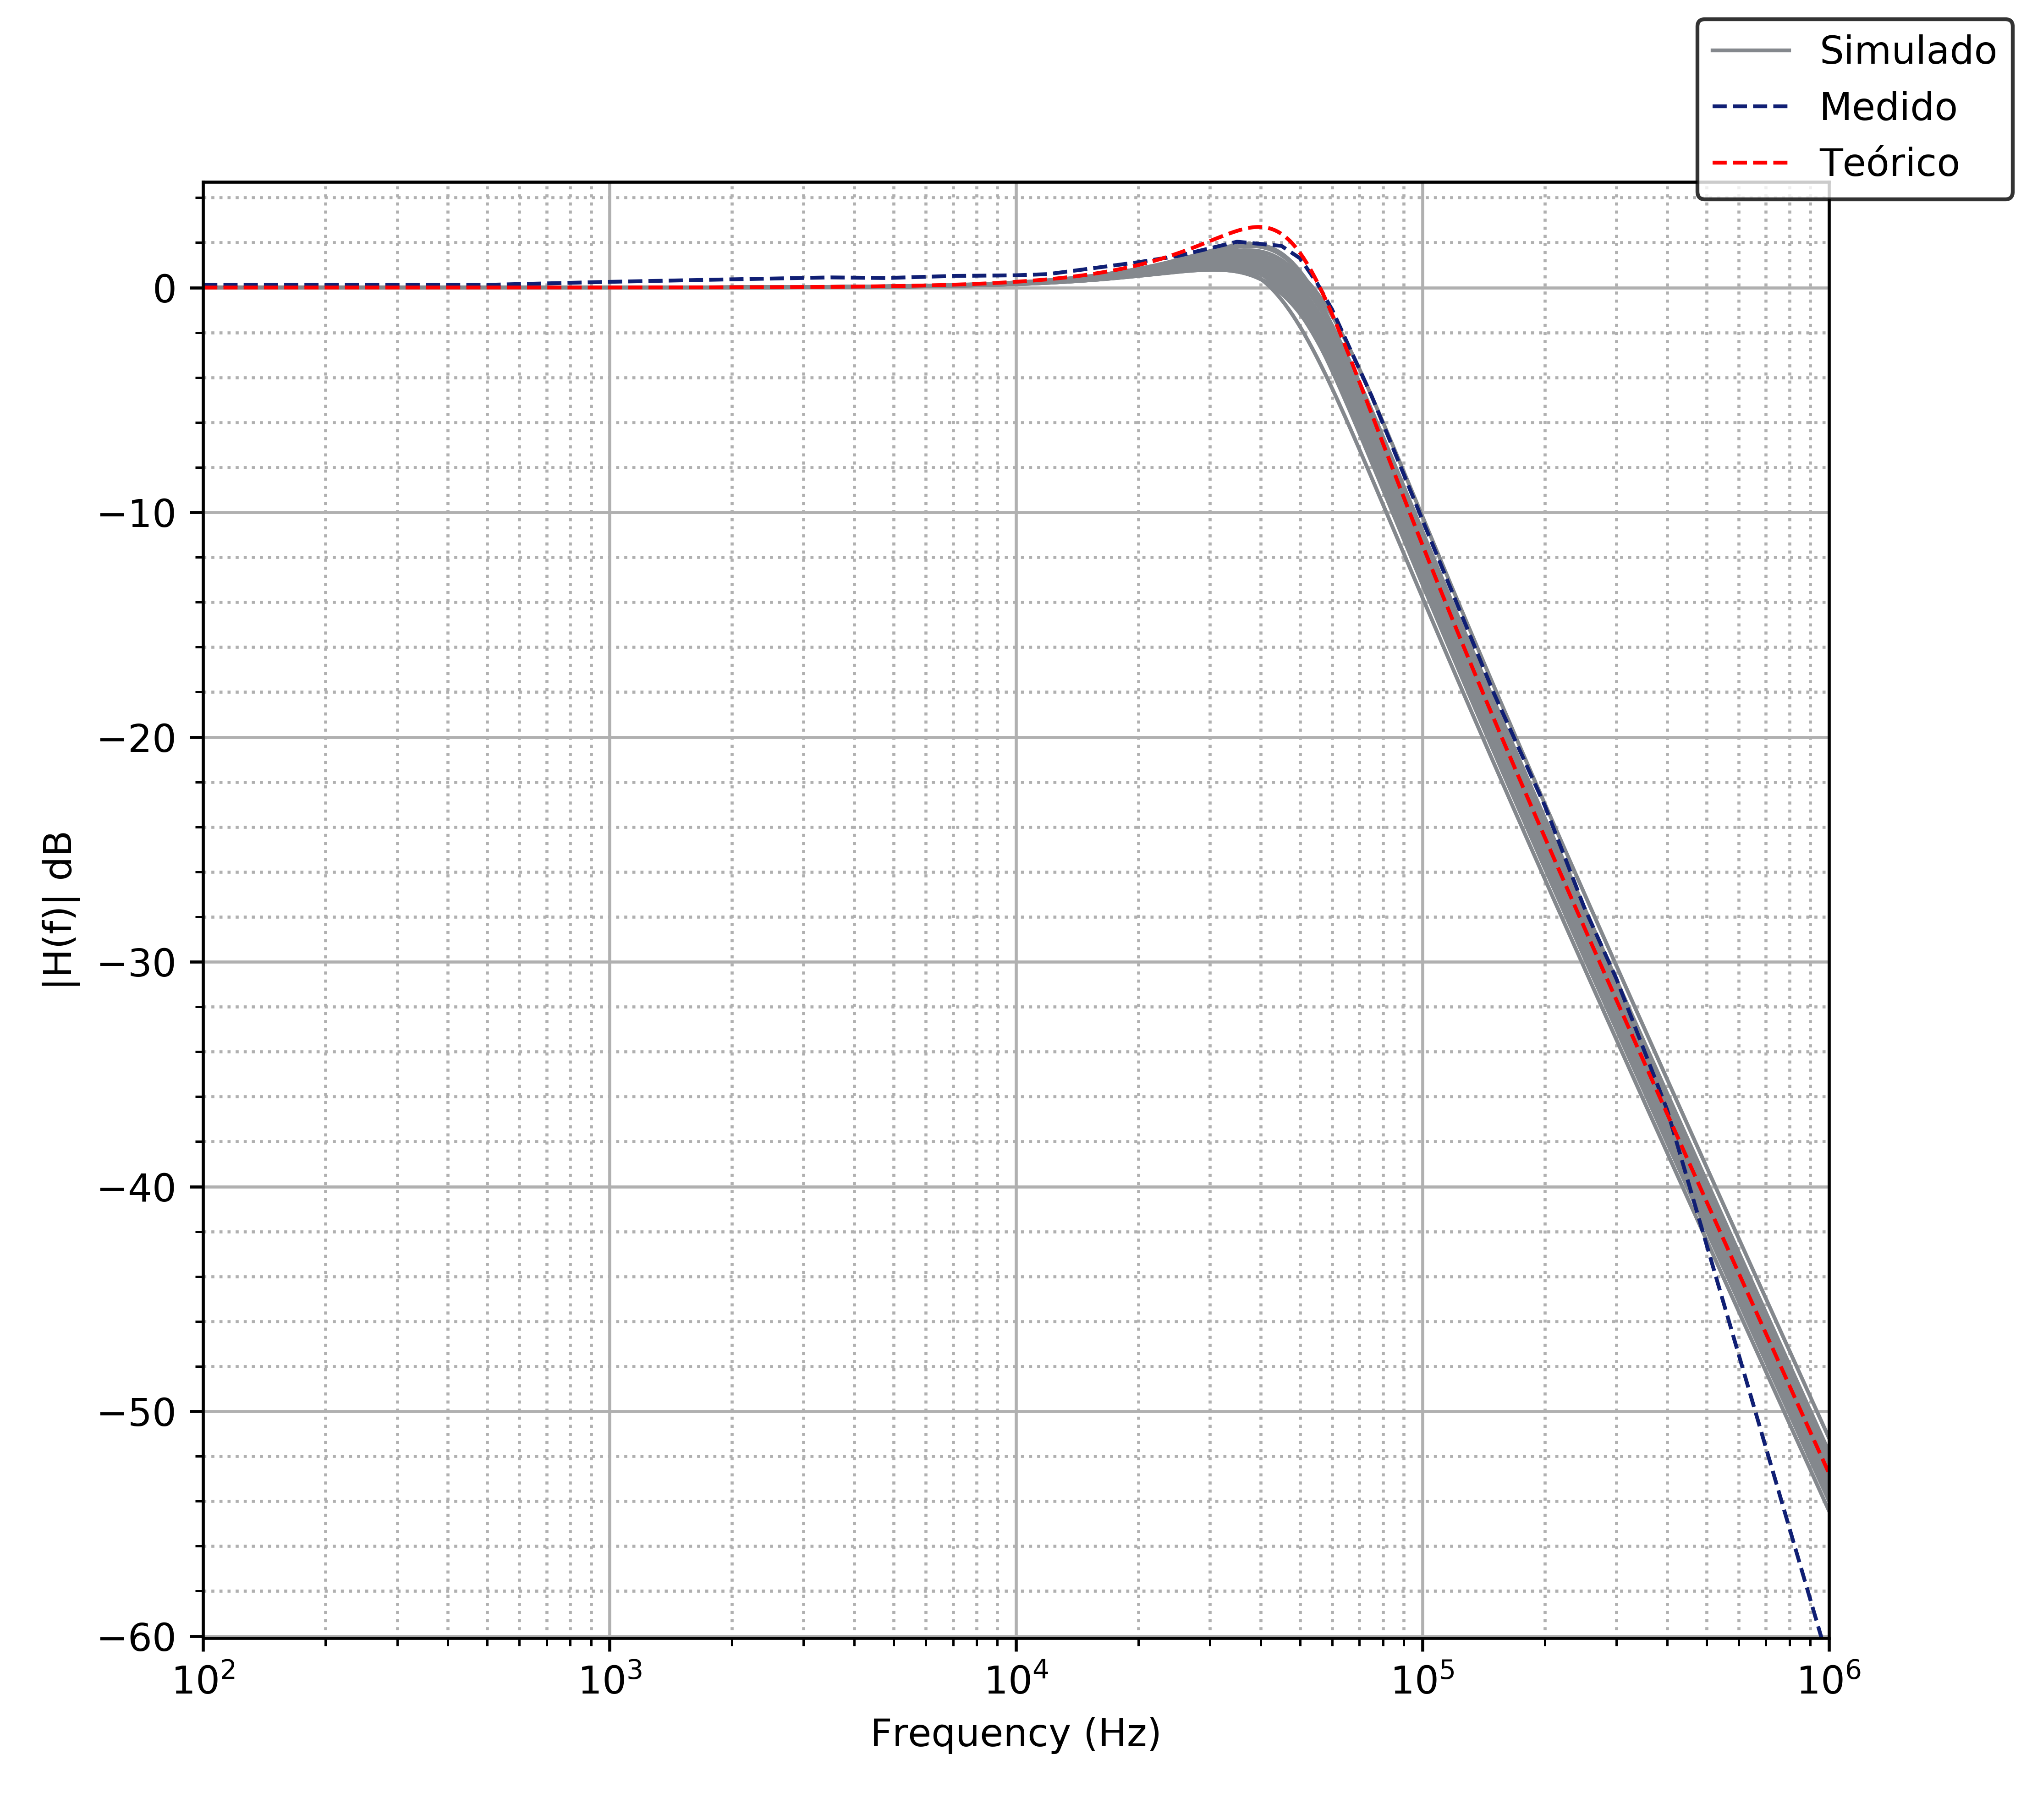
\includegraphics[scale=0.4]{Recursos/pasabajos_plottool_modulo.png}
        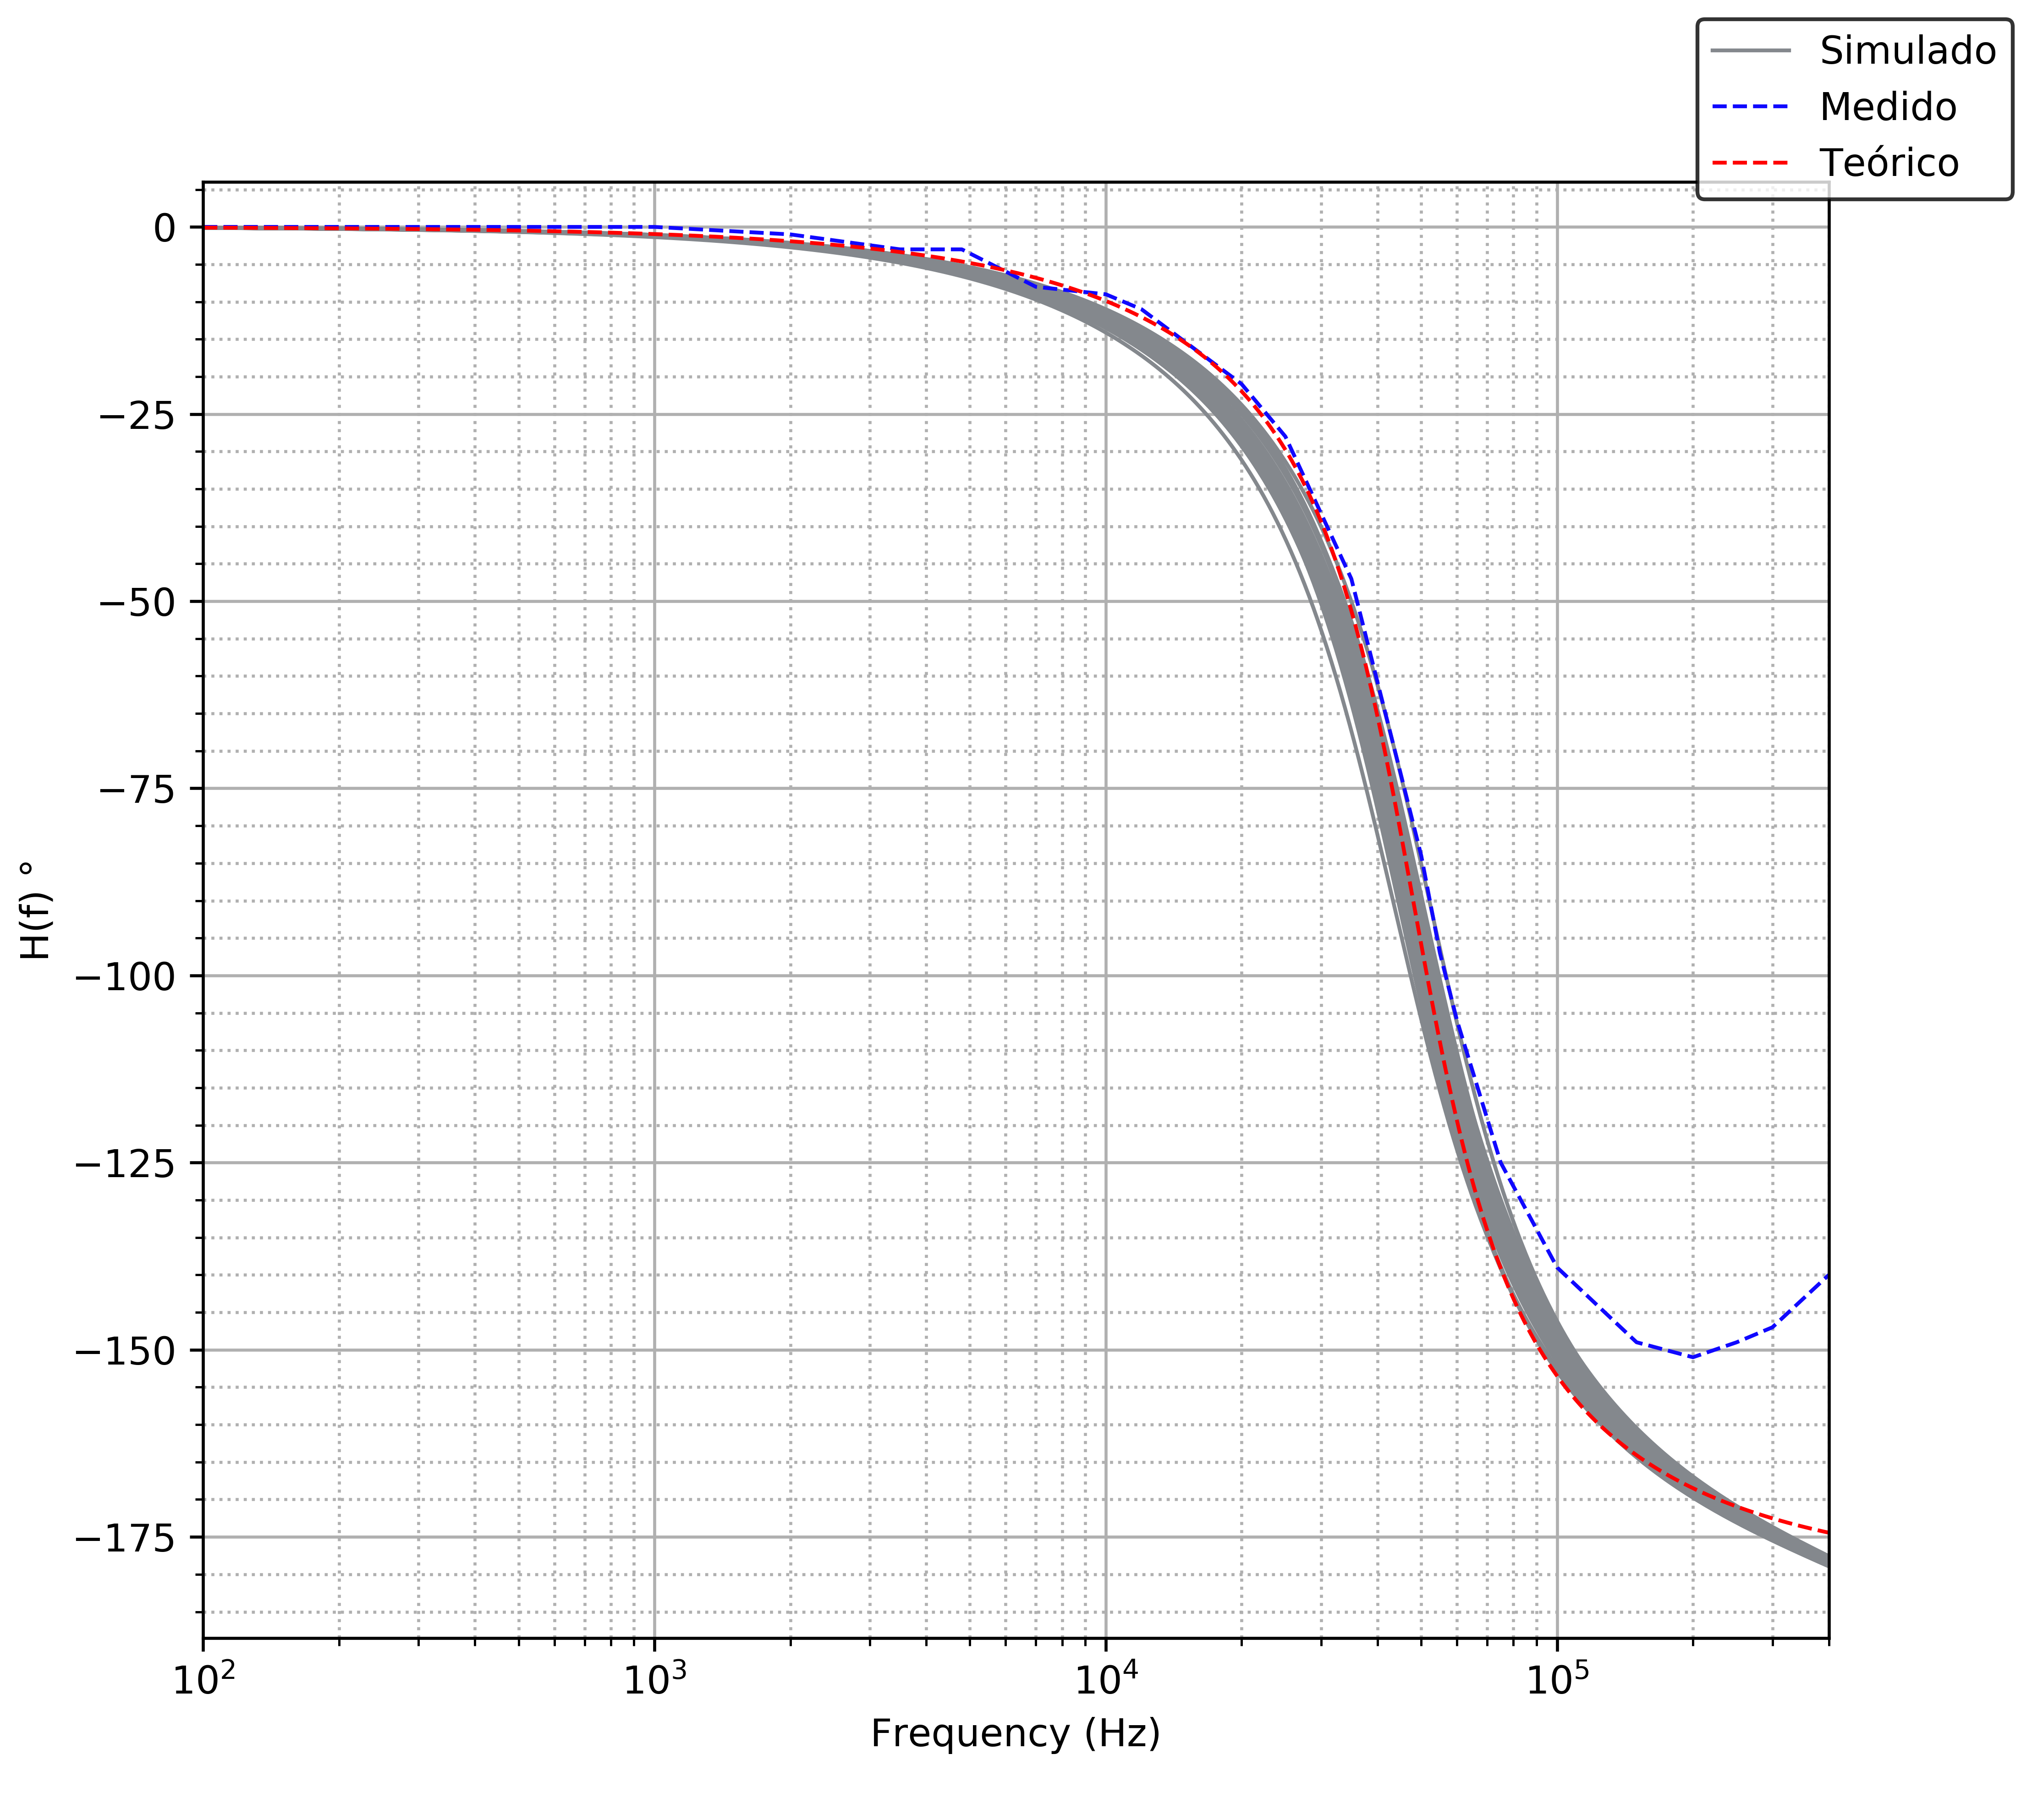
\includegraphics[scale=0.4]{Recursos/pasabajos_plottool_fase.png}
    \end{tabular}
    \caption{Diagramas de bode en m\'odulo y fase del pasabajos}
    \label{fig:respuesta_frecuencia_pasabajos}
\end{figure}


En los gr\'aficos de diagrama de bode de la Fig. \ref{fig:respuesta_frecuencia_pasabajos} se graficaron las curvas propias de la simulaci\'on, la medici\'on y la teor\'ia. Para la simulaci\'on se consider\'o la posible dispersi\'on de los valores
nominales de los componentes seg\'un su tolerancia, de esta forma se puede observar que en un determinado rango de frecuencias las curvas no tienen mucha diferencia, pero sobre todo coinciden en la forma caracter\'istica de la respuesta en frecuencia.

Por otro lado, se puede observar que a partir de una determinada frecuencia, tanto el m\'odulo como la fase de la respuesta en frecuencia que se midi\'o en el circuito empiezan a presentar grandes diferencias con lo te\'orico y lo simulado. Adem\'as, y de hecho lo que resulta m\'as interesante,
es el comportamiento de la fase que aparenta subir a partir de una frecuencia en donde en condiciones te\'oricas deber\'ia seguir decayendo. Para poder explicar esto en principio se busc\'o contemplar alg\'un efecto que pudieran estar agregando las puntas del osciloscopio, pero se descart\'o r\'apidamente
ya que fueron calibradas en x10, con lo cual los efectos par\'asitos comparados contra el capacitor utilizado en la salida no son apreciables. Finalmente, se encontr\'o un sentido cuando se observaron los resultados de analizar las impedancias de los componentes pasivos a diferentes frecuencias y se observ\'o
que el inductor para ciertas frecuencias altas pierde mucho factor de calidad y se comporta como un capacitor. Esto \'ultimo explicar\'ia en principio el hecho de que caiga en m\'odulo la respuesta en frecuencia, puesto que al haber mayor impedancia en la bobina, la ca\'ida en la salida deber\'ia disminuir. Desde otro 
punto de vista, que dejara de comportarse como un inductor producir\'ia que el sistema deje de ser un segundo orden o por lo menos su comportamiento se ver\'a perturbado afectando entonces a la fase de la forma en que lo hace, por culpa del cambio de fase del inductor.